
\section{Conclusions}
This paper presents an end-to-end method for automatic, monocular 3D dog reconstruction. We achieve this using only weak 2D supervision, provided by our novel StanfordExtra dataset. Further, we show we can learn a more detailed shape prior by tuning a gaussian mixture during model training and this leads to improved reconstructions. We also show our method improves over competitive baselines, even when they are given access to ground truth data at test time.

Future work should involve tackling some failure cases of our system, for example handling multiple overlapping dogs or dealing with heavy motion blur. Other areas for research include extending our EM formulation to handle video input to take advantage of multi-view shape constraints, and transferring knowledge accumulated through training on StanfordExtra dogs to other species.

\newcolumntype{?}{!{\vrule width 1pt}}

\newcolumntype{M}[1]{>{\centering\arraybackslash}m{#1}}
\newcommand\scalefactorqual{0.085}
\newcommand\spacerqual{3mm}

\begin{figure*}[t!]
    \centering
    \setkeys{Gin}{width=\linewidth}
    %M{40pt}
    \renewcommand\tabularxcolumn[1]{>{\Centering}m{\scalefactorqual\linewidth}} % set all columns to be centered v & hwise, with a fixed width
    % \begin{tabularx}{\textwidth}{m{15pt}*{5}{X} @ {\hspace{\spacerqual}}*{5}{X}}%
    \begin{tabularx}{\textwidth}{m{15pt}*{5}{X}}
    
        %260pt = 8 rows, 
        \multirow{-2}{*}{\rotatebox[origin=c]{90}{$\overbrace{\hspace{293pt}}^{\textrm{\large StanfordExtra}}$}} &
    
        % R1
        \includegraphics{ours_sup/n02093256-Staffordshire_bullterrier/orig/n02093256_5791.jpg} &
        \includegraphics{ours_sup/n02093256-Staffordshire_bullterrier/fit/n02093256_5791.jpg} &
        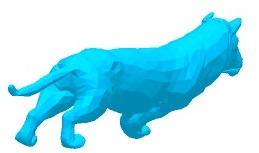
\includegraphics{ours_sup/n02093256-Staffordshire_bullterrier/model/n02093256_5791_crop.jpg} &
        \includegraphics{ours_sup/n02093256-Staffordshire_bullterrier/joints/n02093256_5791.jpg} &
        \includegraphics{ours_sup/n02093256-Staffordshire_bullterrier/segs/n02093256_5791.jpg} \\
        %\hspace{\spacercomp} 
        &\includegraphics{ours_sup/n02088364-beagle/orig/n02088364_2499.jpg} & 
        \includegraphics{ours_sup/n02088364-beagle/fit/n02088364_2499.jpg} & 
        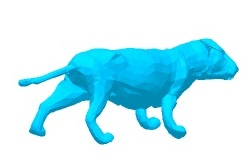
\includegraphics{ours_sup/n02088364-beagle/model/n02088364_2499_crop.jpg} & 
        \includegraphics{ours_sup/n02088364-beagle/joints/n02088364_2499.jpg} & 
        \includegraphics{ours_sup/n02088364-beagle/segs/n02088364_2499.jpg} \\ 

        % R2
        &\includegraphics{ours_sup/n02107908-Appenzeller/orig/n02107908_933.jpg} & 
        \includegraphics{ours_sup/n02107908-Appenzeller/fit/n02107908_933.jpg} & 
        \includegraphics{ours_sup/n02107908-Appenzeller/model/n02107908_933.jpg} & 
        \includegraphics{ours_sup/n02107908-Appenzeller/joints/n02107908_933.jpg} & 
        \includegraphics{ours_sup/n02107908-Appenzeller/segs/n02107908_933.jpg} \\
        %\hspace{\spacercomp} 
        &\includegraphics{ours_sup/n02088094-Afghan_hound/orig/n02088094_1917.jpg} & 
        \includegraphics{ours_sup/n02088094-Afghan_hound/fit/n02088094_1917.jpg} & 
        \includegraphics{ours_sup/n02088094-Afghan_hound/model/n02088094_1917.jpg} & 
        \includegraphics{ours_sup/n02088094-Afghan_hound/joints/n02088094_1917.jpg} & 
        \includegraphics{ours_sup/n02088094-Afghan_hound/segs/n02088094_1917.jpg} \\ 

        % R3
        &\includegraphics{ours_sup/n02087394-Rhodesian_ridgeback/orig/n02087394_7056.jpg} & 
        \includegraphics{ours_sup/n02087394-Rhodesian_ridgeback/fit/n02087394_7056.jpg} & 
        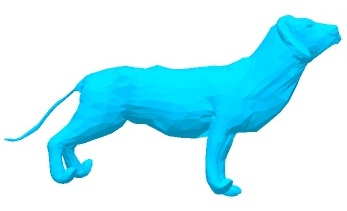
\includegraphics{ours_sup/n02087394-Rhodesian_ridgeback/model/n02087394_7056_crop.jpg} & 
        \includegraphics{ours_sup/n02087394-Rhodesian_ridgeback/joints/n02087394_7056.jpg} & 
        \includegraphics{ours_sup/n02087394-Rhodesian_ridgeback/segs/n02087394_7056.jpg} \\
        %\hspace{\spacercomp} 
        &\includegraphics{ours_sup/n02099601-golden_retriever/orig/n02099601_304.jpg} & 
        \includegraphics{ours_sup/n02099601-golden_retriever/fit/n02099601_304.jpg} & 
        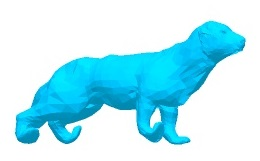
\includegraphics{ours_sup/n02099601-golden_retriever/model/n02099601_304_crop.jpg} & 
        \includegraphics{ours_sup/n02099601-golden_retriever/joints/n02099601_304.jpg} & 
        \includegraphics{ours_sup/n02099601-golden_retriever/segs/n02099601_304.jpg} \\ 
        
        % R4
        &\includegraphics{ours_sup/n02085620-Chihuahua/orig/n02085620_3651.jpg} & 
        \includegraphics{ours_sup/n02085620-Chihuahua/fit/n02085620_3651.jpg} & 
        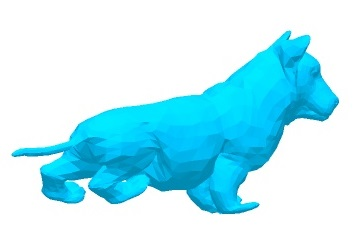
\includegraphics{ours_sup/n02085620-Chihuahua/model/n02085620_3651_crop.jpg} &
        \includegraphics{ours_sup/n02085620-Chihuahua/joints/n02085620_3651.jpg} &
        \includegraphics{ours_sup/n02085620-Chihuahua/segs/n02085620_3651.jpg} \\
        %\hspace{\spacercomp} 
        % \includegraphics{ours_sup/n02091134-whippet/orig/n02091134_16201.jpg} &
        % \includegraphics{ours_sup/n02091134-whippet/fit/n02091134_16201.jpg} &
        % \includegraphics{ours_sup/n02091134-whippet/model/n02091134_16201.jpg} &
        % \includegraphics{ours_sup/n02091134-whippet/joints/n02091134_16201.jpg} &
        % \includegraphics{ours_sup/n02091134-whippet/segs/n02091134_16201.jpg} \\ 
        &\includegraphics{ours_sup/n02097130-giant_schnauzer/orig/n02097130_5121.jpg} &
        \includegraphics{ours_sup/n02097130-giant_schnauzer/fit/n02097130_5121.jpg} &
        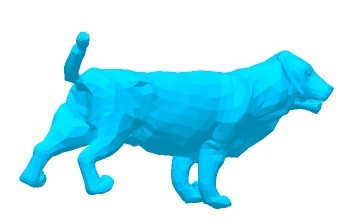
\includegraphics{ours_sup/n02097130-giant_schnauzer/model/n02097130_5121_crop.jpg} &
        \includegraphics{ours_sup/n02097130-giant_schnauzer/joints/n02097130_5121.jpg} &
        \includegraphics{ours_sup/n02097130-giant_schnauzer/segs/n02097130_5121.jpg} \\
        
        % R5
        &\includegraphics{ours_sup/n02089078-black-and-tan_coonhound/orig/n02089078_877.jpg} &
        \includegraphics{ours_sup/n02089078-black-and-tan_coonhound/fit/n02089078_877.jpg} &
        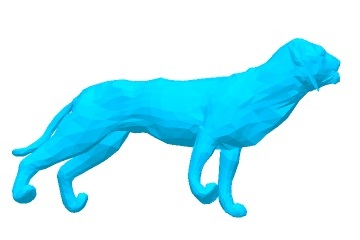
\includegraphics{ours_sup/n02089078-black-and-tan_coonhound/model/n02089078_877_crop.jpg} &
        \includegraphics{ours_sup/n02089078-black-and-tan_coonhound/joints/n02089078_877.jpg} &
        \includegraphics{ours_sup/n02089078-black-and-tan_coonhound/segs/n02089078_877.jpg} \\
        %\hspace{\spacercomp} 
        &\includegraphics{ours_sup/n02085620-Chihuahua/orig/n02085620_1152.jpg} &
        \includegraphics{ours_sup/n02085620-Chihuahua/fit/n02085620_1152.jpg} &
        \includegraphics{ours_sup/n02085620-Chihuahua/model/n02085620_1152_crop.jpg} &
        \includegraphics{ours_sup/n02085620-Chihuahua/joints/n02085620_1152.jpg} &
        \includegraphics{ours_sup/n02085620-Chihuahua/segs/n02085620_1152.jpg} \\ 
        
        % R6
        &\includegraphics{ours_sup/n02108000-EntleBucher/orig/n02108000_3104.jpg} &
        \includegraphics{ours_sup/n02108000-EntleBucher/fit/n02108000_3104.jpg} &
        \includegraphics{ours_sup/n02108000-EntleBucher/model/n02108000_3104_crop.jpg} &
        \includegraphics{ours_sup/n02108000-EntleBucher/joints/n02108000_3104.jpg} &
        \includegraphics{ours_sup/n02108000-EntleBucher/segs/n02108000_3104.jpg} \\
        %\hspace{\spacercomp} 
        &\includegraphics{ours_sup/n02105162-malinois/orig/n02105162_688.jpg} &
        \includegraphics{ours_sup/n02105162-malinois/fit/n02105162_688.jpg} &
        \includegraphics{ours_sup/n02105162-malinois/model/n02105162_688_crop.jpg} &
        \includegraphics{ours_sup/n02105162-malinois/joints/n02105162_688.jpg} &
        \includegraphics{ours_sup/n02105162-malinois/segs/n02105162_688.jpg} \\ 
        
        % R7
        &\includegraphics{ours_sup/n02102318-cocker_spaniel/orig/n02102318_11648.jpg} &
        \includegraphics{ours_sup/n02102318-cocker_spaniel/fit/n02102318_11648.jpg} &
        \includegraphics{ours_sup/n02102318-cocker_spaniel/model/n02102318_11648_crop.jpg} &
        \includegraphics{ours_sup/n02102318-cocker_spaniel/joints/n02102318_11648.jpg} &
        \includegraphics{ours_sup/n02102318-cocker_spaniel/segs/n02102318_11648.jpg} \\
        %\hspace{\spacercomp}
        &\includegraphics{ours_sup/n02086910-papillon/orig/n02086910_3020.jpg} &
        \includegraphics{ours_sup/n02086910-papillon/fit/n02086910_3020.jpg} &
        \includegraphics{ours_sup/n02086910-papillon/model/n02086910_3020_crop.jpg} &
        \includegraphics{ours_sup/n02086910-papillon/joints/n02086910_3020.jpg} &
        \includegraphics{ours_sup/n02086910-papillon/segs/n02086910_3020.jpg} \\
        
        % R8
        % &\includegraphics{ours_sup/n02097130-giant_schnauzer/orig/n02097130_5121.jpg} &
        % \includegraphics{ours_sup/n02097130-giant_schnauzer/fit/n02097130_5121.jpg} &
        % \includegraphics{ours_sup/n02097130-giant_schnauzer/model/n02097130_5121.jpg} &
        % \includegraphics{ours_sup/n02097130-giant_schnauzer/joints/n02097130_5121.jpg} &
        % \includegraphics{ours_sup/n02097130-giant_schnauzer/segs/n02097130_5121.jpg} &
        % \hspace{\spacercomp} 
        % \includegraphics{ours_sup/n02087394-Rhodesian_ridgeback/orig/n02087394_831.jpg} &
        % \includegraphics{ours_sup/n02087394-Rhodesian_ridgeback/fit/n02087394_831.jpg} &
        % \includegraphics{ours_sup/n02087394-Rhodesian_ridgeback/model/n02087394_831.jpg} &
        % \includegraphics{ours_sup/n02087394-Rhodesian_ridgeback/joints/n02087394_831.jpg} &
        % \includegraphics{ours_sup/n02087394-Rhodesian_ridgeback/segs/n02087394_831.jpg} \\

        % R9
        &\includegraphics{ours_sup/n02091032-Italian_greyhound/orig/n02091032_1933.jpg} &
        \includegraphics{ours_sup/n02091032-Italian_greyhound/fit/n02091032_1933.jpg} &
        \includegraphics{ours_sup/n02091032-Italian_greyhound/model/n02091032_1933_crop.jpg} &
        \includegraphics{ours_sup/n02091032-Italian_greyhound/joints/n02091032_1933.jpg} &
        \includegraphics{ours_sup/n02091032-Italian_greyhound/segs/n02091032_1933.jpg} \\
        %\hspace{\spacercomp}
        &\includegraphics{ours_sup/n02093647-Bedlington_terrier/orig/n02093647_3594.jpg} &
        \includegraphics{ours_sup/n02093647-Bedlington_terrier/fit/n02093647_3594.jpg} &
        \includegraphics{ours_sup/n02093647-Bedlington_terrier/model/n02093647_3594_crop.jpg} &
        \includegraphics{ours_sup/n02093647-Bedlington_terrier/joints/n02093647_3594.jpg} &
        \includegraphics{ours_sup/n02093647-Bedlington_terrier/segs/n02093647_3594.jpg} \\

        %R10
        &\includegraphics{ours_sup/n02106662-German_shepherd/orig/n02106662_13599.jpg} &
        \includegraphics{ours_sup/n02106662-German_shepherd/fit/n02106662_13599.jpg} &
        \includegraphics{ours_sup/n02106662-German_shepherd/model/n02106662_13599_crop.jpg} &
        \includegraphics{ours_sup/n02106662-German_shepherd/joints/n02106662_13599.jpg} &
        \includegraphics{ours_sup/n02106662-German_shepherd/segs/n02106662_13599.jpg} \\
        %\hspace{\spacercomp} 
        &\includegraphics{ours_sup/n02095314-wire-haired_fox_terrier/orig/n02095314_261.jpg} &
        \includegraphics{ours_sup/n02095314-wire-haired_fox_terrier/fit/n02095314_261.jpg} &
        \includegraphics{ours_sup/n02095314-wire-haired_fox_terrier/model/n02095314_261.jpg} &
        \includegraphics{ours_sup/n02095314-wire-haired_fox_terrier/joints/n02095314_261.jpg} &
        \includegraphics{ours_sup/n02095314-wire-haired_fox_terrier/segs/n02095314_261.jpg} \\

        % R11
        \multirow{-2.1}{*}{\rotatebox[origin=c]{90}{$\overbrace{\hspace{64pt}}^{\textrm{\large Animal Pose}}$}} &
        
        \includegraphics{ours_sup/animal_pose_fits/orig/2007_000063.jpg} &
        \includegraphics{ours_sup/animal_pose_fits/fit/2007_000063.jpg} &
        \includegraphics{ours_sup/animal_pose_fits/model/2007_000063_crop.jpg} &
        \includegraphics{ours_sup/animal_pose_fits/joints/2007_000063.jpg} &
        \includegraphics{ours_sup/animal_pose_fits/segs/2007_000063.jpg} \\
        %\hspace{\spacercomp} 
        &\includegraphics{ours_sup/animal_pose_fits/orig/2007_004189.jpg} &
        \includegraphics{ours_sup/animal_pose_fits/fit/2007_004189.jpg} &
        \includegraphics{ours_sup/animal_pose_fits/model/2007_004189_crop.jpg} &
        \includegraphics{ours_sup/animal_pose_fits/joints/2007_004189.jpg} &
        \includegraphics{ours_sup/animal_pose_fits/segs/2007_004189.jpg} \\ 

        % R12
        &\includegraphics{ours_sup/animal_pose_fits/orig/2007_008222.jpg} &
        \includegraphics{ours_sup/animal_pose_fits/fit/2007_008222.jpg} &
        \includegraphics{ours_sup/animal_pose_fits/model/2007_008222_crop.jpg} &
        \includegraphics{ours_sup/animal_pose_fits/joints/2007_008222.jpg} &
        \includegraphics{ours_sup/animal_pose_fits/segs/2007_008222.jpg} \\
        %\hspace{\spacercomp} 
        \includegraphics{ours_sup/animal_pose_fits/orig/2007_009605.jpg} &
        \includegraphics{ours_sup/animal_pose_fits/fit/2007_009605.jpg} &
        \includegraphics{ours_sup/animal_pose_fits/model/2007_009605_crop.jpg} &
        \includegraphics{ours_sup/animal_pose_fits/joints/2007_009605.jpg} &
        \includegraphics{ours_sup/animal_pose_fits/segs/2007_009605.jpg} \\ 
        
        & (a) & (b) & (c) & (d) & (e) \\
        %\hspace{\spacercomp} 
        % (a) & (b) & (c) & (d) & (e) \\

    \end{tabularx}
    %
    \caption{%
    \textbf{Qualitative results on StanfordExtra and Animal Pose~\cite{animalpose}.} 
        For each sample we show: (a) input image, (b) predicted 3D mesh, 
        (c) canonical view 3D mesh, (d) reprojected model joints and 
        (e) silhouette reprojection error.
    }
    \label{fig:qualresults_sup}
\end{figure*}
